\documentclass[a4paper,12pt]{article}
\usepackage[english]{babel}
\usepackage[utf8x]{inputenc}
\usepackage{amsmath, epic, eepic, float, subfig, amsfonts, color, amsthm, textcomp, microtype, fullpage}
\usepackage[parfill]{parskip}
\usepackage[pdftex]{graphicx}
\usepackage{color}
\usepackage[linkcolor=black,urlcolor=blue,citecolor=black]{hyperref}
\hypersetup{colorlinks=true}
\newcommand{\HRule}{\rule{\linewidth}{0.5mm}}

\begin{document}
\begin{titlepage}
\begin{center}
\includegraphics[width=0.5\textwidth]{./logo.pdf}~\\[1cm]


\textsc{\Large Ethiek 1}\\[0.5cm]

\HRule \\[0.4cm]
{ \LARGE \bfseries Project empathie in de sociale sector}\\[0.4cm]
{\large \emph{'t Wit Huis, Loppem}}\\[0.2cm]

\HRule \\[1.5cm]

\begin{minipage}{0.4\textwidth}
\begin{flushleft} \large
\emph{door:}\\
Haroen \textsc{Viaene}\\

\end{flushleft}
\end{minipage}
\begin{minipage}{0.4\textwidth}
\begin{flushright} \large
\large{2$^{\text{de}}$ fase bachelor Elektronica-ICT}\\
\end{flushright}
\end{minipage}

\vfill

{\large 2015-2016}

\end{center}
\end{titlepage}

\newpage

\section*{Inhoud}

% maak Nederlandstalig
\tableofcontents

\newpage

\section{Voorstelling}

% voorstelling van de instelling, de doelgroep, met contactpersoon, 1 bladzijde

\emph{’t Wit Huis} te Loppem is een voorziening van het type ``werken en wonen'' voor volwassen personen met een meervoudige handicap. In de meeste gevallen is dit een visuele handicap gecombineerd met een verstandelijke of motorische. De meeste van de bewoners blijven er permanent, maar er zijn er ook een aantal die enkele dagen per week ergens anders werken of verblijven.

De voorziening maakt deel uit van de organisatie Spermalie, en daarbinnen De Kade.

\emph{’t Wit Huis} volgt de psychoanalytische werkvisie van Jacques Lacan. Deze visie gaat ervan uit dat we allemaal ons eigen geluk zelf kunnen vinden. Daarom wordt er hier zo veel mogelijk ruimte gelaten voor vrije tijd en voor creativiteit binnen de activiteiten. Zo zal er nooit gezegd worden ``We zullen nu dit liedje van die artiest spelen'', maar wel ``Welk liedje dat je geschreven hebt gaan we nu spelen, Peter?''.

De activiteiten zijn zeer gevarieerd, en meestal op het creatieve vlak van de bewoners gericht. Zo is er een muziekgroep ``De Witte Wolven''(vroeger ``White House Band''), die vroeger enkele cd's uitgebracht heeft en ook samen gewerkt heeft met o.a. Wigbert en Wim Opbrouck. Verder is er recent een gedichtenbundel uitgebracht, een zeer actieve beeldentuin met werken van bekende kunstenaars van over de wereld gecombineerd met de werken die door de bewoners zelf worden gemaakt. Deze werken worden ook over het hele centrum tentoon gesteld.

Ook wordt er door de voorziening ergotherapie georganiseerd. Dit zijn activiteiten zoals boetseren, potten maken, papier scheppen, kaartjes maken, bloemschikken, thee, zeep, shampoos; maar ook eieren, fruit- en groenteteelt, pizza's en lasagne gemaakt om te verkopen aan buitenstaanders. Zo worden mensen zo vaak mogelijk betrokken binnen de organisatie, dit kadert in een een visie waarin er zoveel mogelijk aan integratie gewerkt wordt. Bewoners die hiertoe in staat zijn gaan ook bijvoorbeeld om hun eigen boodschappen.

Op iets praktischer vlak helpen de bewoners ook mee met het repareren van bepaalde gebroken dingen, vogelnestjes maken, vroeger ook helpen met het eten (maar dit is tegenwoordig niet meer toegelaten door strengere eisen qua voedsel).

Ook is er een grote focus op sport, en wordt er ook elk jaar meegedaan aan evenementen zoals de Special Olympics en lokale fiets-, loop-, zwem- en andere wedstrijden.

Buiten sportwedstrijden wordt er ook na de activiteiten---al dan niet met vrijwilligers---aan sport zoals fietsen met tandems, fitness, wandelen enz. gedaan.

Er worden ook vaak uitstappen georganiseerd, zoals laatst naar toneeloptredens, volksspelen, bibliotheken en ook op reis gegaan. Zo zijn ze al naar Engeland, Lourdes \dots gegaan.

De bewoners kunnen elk jaar een programma beslissen, met activiteiten die voorgesteld worden door de begeleiders zelf. Tijdens hun vrije tijd mogen ze in hun zelf versierde kamer verblijven, maar ook in de gemeenschappelijke ruimtes kom je altijd wel een aantal bewoners tegen.

Op \emph{'t Wit Huis} verblijven momenteel 33 bewoners van 19 tot 75 jaar. Ze worden begeleid door 30-tal begeleiders.

Mijn initiële contactpersoon in deze voorziening is mijn vader, Geert Viaene, maar tijdens de stage volg ik ook de activiteiten van Jürgen Tierlinckx en Bart% check %
. \emph{'t Wit Huis} bevindt zich in de Rijselsestraat 13, 8200 Loppem.

\section{Verslag}

% per uur, concreet, drie bladzijden

\subsection{Maandag 14 december 2015}

\subsubsection{Voormiddag}

Ik ben toegekomen per fiets om iets na 8:00 's morgens. De echte werkdag begon een halfuur later, terwijl ik daarop wacht, loop ik al eens rond met mijn vader, die me kennis doet maken met de bewoners. Nadat dat gebeurd was, ging ik terug naar de personeelsruimte, en vertrok mijn vader naar huis; hij moet vandaag niet werken.

Rond 8:30 begint de vergadering, waarvan ik uiteraard niets mag vertellen in dit verslag. Hier kreeg ik mijn taak voor de dag en de volgende dagen, namelijk deze morgen \emph{klusklub}, in de namiddag \emph{wandelen}, morgen \emph{muziek} en in de namiddag \emph{bewonersvergadering} (voor de meeste andere begeleiders is het dan vergadering waar ik niet aan meedoe). Volgende maandag is het hetzelfde programma als vandaag.

Ik volg deze morgen opvoeder Jürgen Tierlinkx. We beginnen met de drie bewoners waarbij hij de \emph{morgengroet} doet. Dit is redelijk simpel aangezien het opstaan relatief autonoom gebeurt (of misschien tijdens de nachtshift, ik ben het niet helemaal zeker). De taak die hierbij hoort is eigenlijk redelijk gemakkelijk, en bestaat uit het controleren dat die bewoners effectief aanwezig zijn, hun bet effectief gemaakt is en ze geschoren zijn en hun tanden gepoetst hebben. Dit gebeurde aan een redelijk laid-back tempo, waardoor het ongeveer 10:00 was toen we begonnen met de activiteit.

De activiteit in de morgen heette \emph{klusklub}, waarbij een aantal bewoners meehelpen met enkele klusjes die nodig zijn in het gebouw. Dit kunnen dingen zijn als gebroken toestellen repareren, of zoals nu een verbetering ergens aan toevoegen.

Vandaag was dit het toevoegen aan blokjes in een sportrek. Er hing een ijzeren rek aan de hoogste sport voor de opening die zo'n sportrek altijd heeft. Dit was jammer genoeg te laag voor enkele bewoners dus moest het verplaatst worden naar de hoogste sport. Op die hoogte waren er geen sporten onder voor het te ondersteunen, dus dat moest vervangen worden door blokjes. De materialen hebben we gehaald bij de houtwerkplaats, die deze instelling ook heeft.

Dit werk was rond 11:45 gedaan, waarna ik geholpen heb bij het sorteren van het eten---dat via Spermalie geregeld wordt. Bij het eten heb ik geholpen bij het inschenken van mijn tafel, opscheppen van de borden en bij één iemand moest het eten voor hem gesneden worden.

Om 13:12 was mijn werk gedaan, en heb ik het evaluatieblad afgegeven aan de groepschef van de instelling. Daarna heb ik mijn verslag van de voormiddag geschreven. Om 13:30 begint de vergadering die de namiddag doet opstarten.

\subsubsection{Namiddag}

De middag begint net zoals de voormiddag met een vergadering van $\pm$ 25 minuten. Deze overloopt opnieuw elk van de bewoners, en zegt nog even snel hoe de taken verdeeld zijn.

In de namiddag volg ik opvoeder Bart, die zal wandelen. We gaan naar Zevenkerke, waar we wandelen van 14:00 tot 15:30. Bij deze activiteit was er ook een andere vrijwilliger aanwezig die vaker meegaat. Bij het wandelen heb ik gepraat met alle vier de bewoners die mee gingen. Uit respect voor de privacy van de bewoners zal ik hier niet te diep op ingaan, maar ik heb toch een aantal keer moeten uitleggen dat ik dit verslag nu moest schrijven, en \emph{waarom} ik nu eigenlijk een stage doe voor 24 uur als ik geen gerelateerde richting doe.

Ik vond het ook interessant om te horen hoe mensen die een heel anders profiel hebben dan de meeste mensen toch nog vergelijkbare gedachten hebben als anderen.

Na het wandelen drinken we allemaal een drankje in de cafetaria van de Abdij van Zevenkerke. Bij het terug aankomen in de instelling praat ik nog met een bewoner die wel drie dagen per week thuisblijft, hij werkt bij een woonzorgcentrum in de buurt bij de afwas.

Om 16:45 heb ik mijn dag afgesloten en ben ik naar huis gegaan.

\subsection{Dinsdag 15 december 2015}

\subsubsection{Voormiddag}

Deze dag begon net zoals gisteren met de vergadering die alle bewoners en de taken overloopt. Deze duurt van 8:30 tot 9:00. Hierin wordt nog eens bevestigd dat ik deze morgen de activiteit \emph{muziek} volg. Deze wordt begeleid door Geert Viaene. Het is leuk om de bewoners in deze context te zien verademen en veel van hun creatieve energie kwijt te raken.

Zoals eerder al gezegd zijn er al cd's opgenomen in het verleden, en nu werken ze aan nieuwe opnames. Een vrijwilliger die een eigen studio heeft zal helpen met het opnemen ervan.

De bewoners schrijven hun eigen nummers, die vaak gaan over liefde, dingen die ze tegenkomen tijdens de dagelijkse sleur. Enkele bewoners zingen ook over de dingen die ze herinneren van voor ze hier verbleven, van toen ze een \emph{normaler} leven hadden.

Tijdens deze activiteit was er een grote vraag vanuit de bewoners dat ik ook op de \emph{batphone} (een soort panfluit, maar dan met elk van de buizen met een diameter van tien centimeter, en één tot anderhalve meter lang, je bespeelt het met een soort pingpongpalletjes gemaakt uit foam) speelde en meezong. Ik merkte dat ze door hun meestal visuele handicap een uitzonderlijk goed ritmegevoel hebben.

\begin{figure}[H]
  \centering
  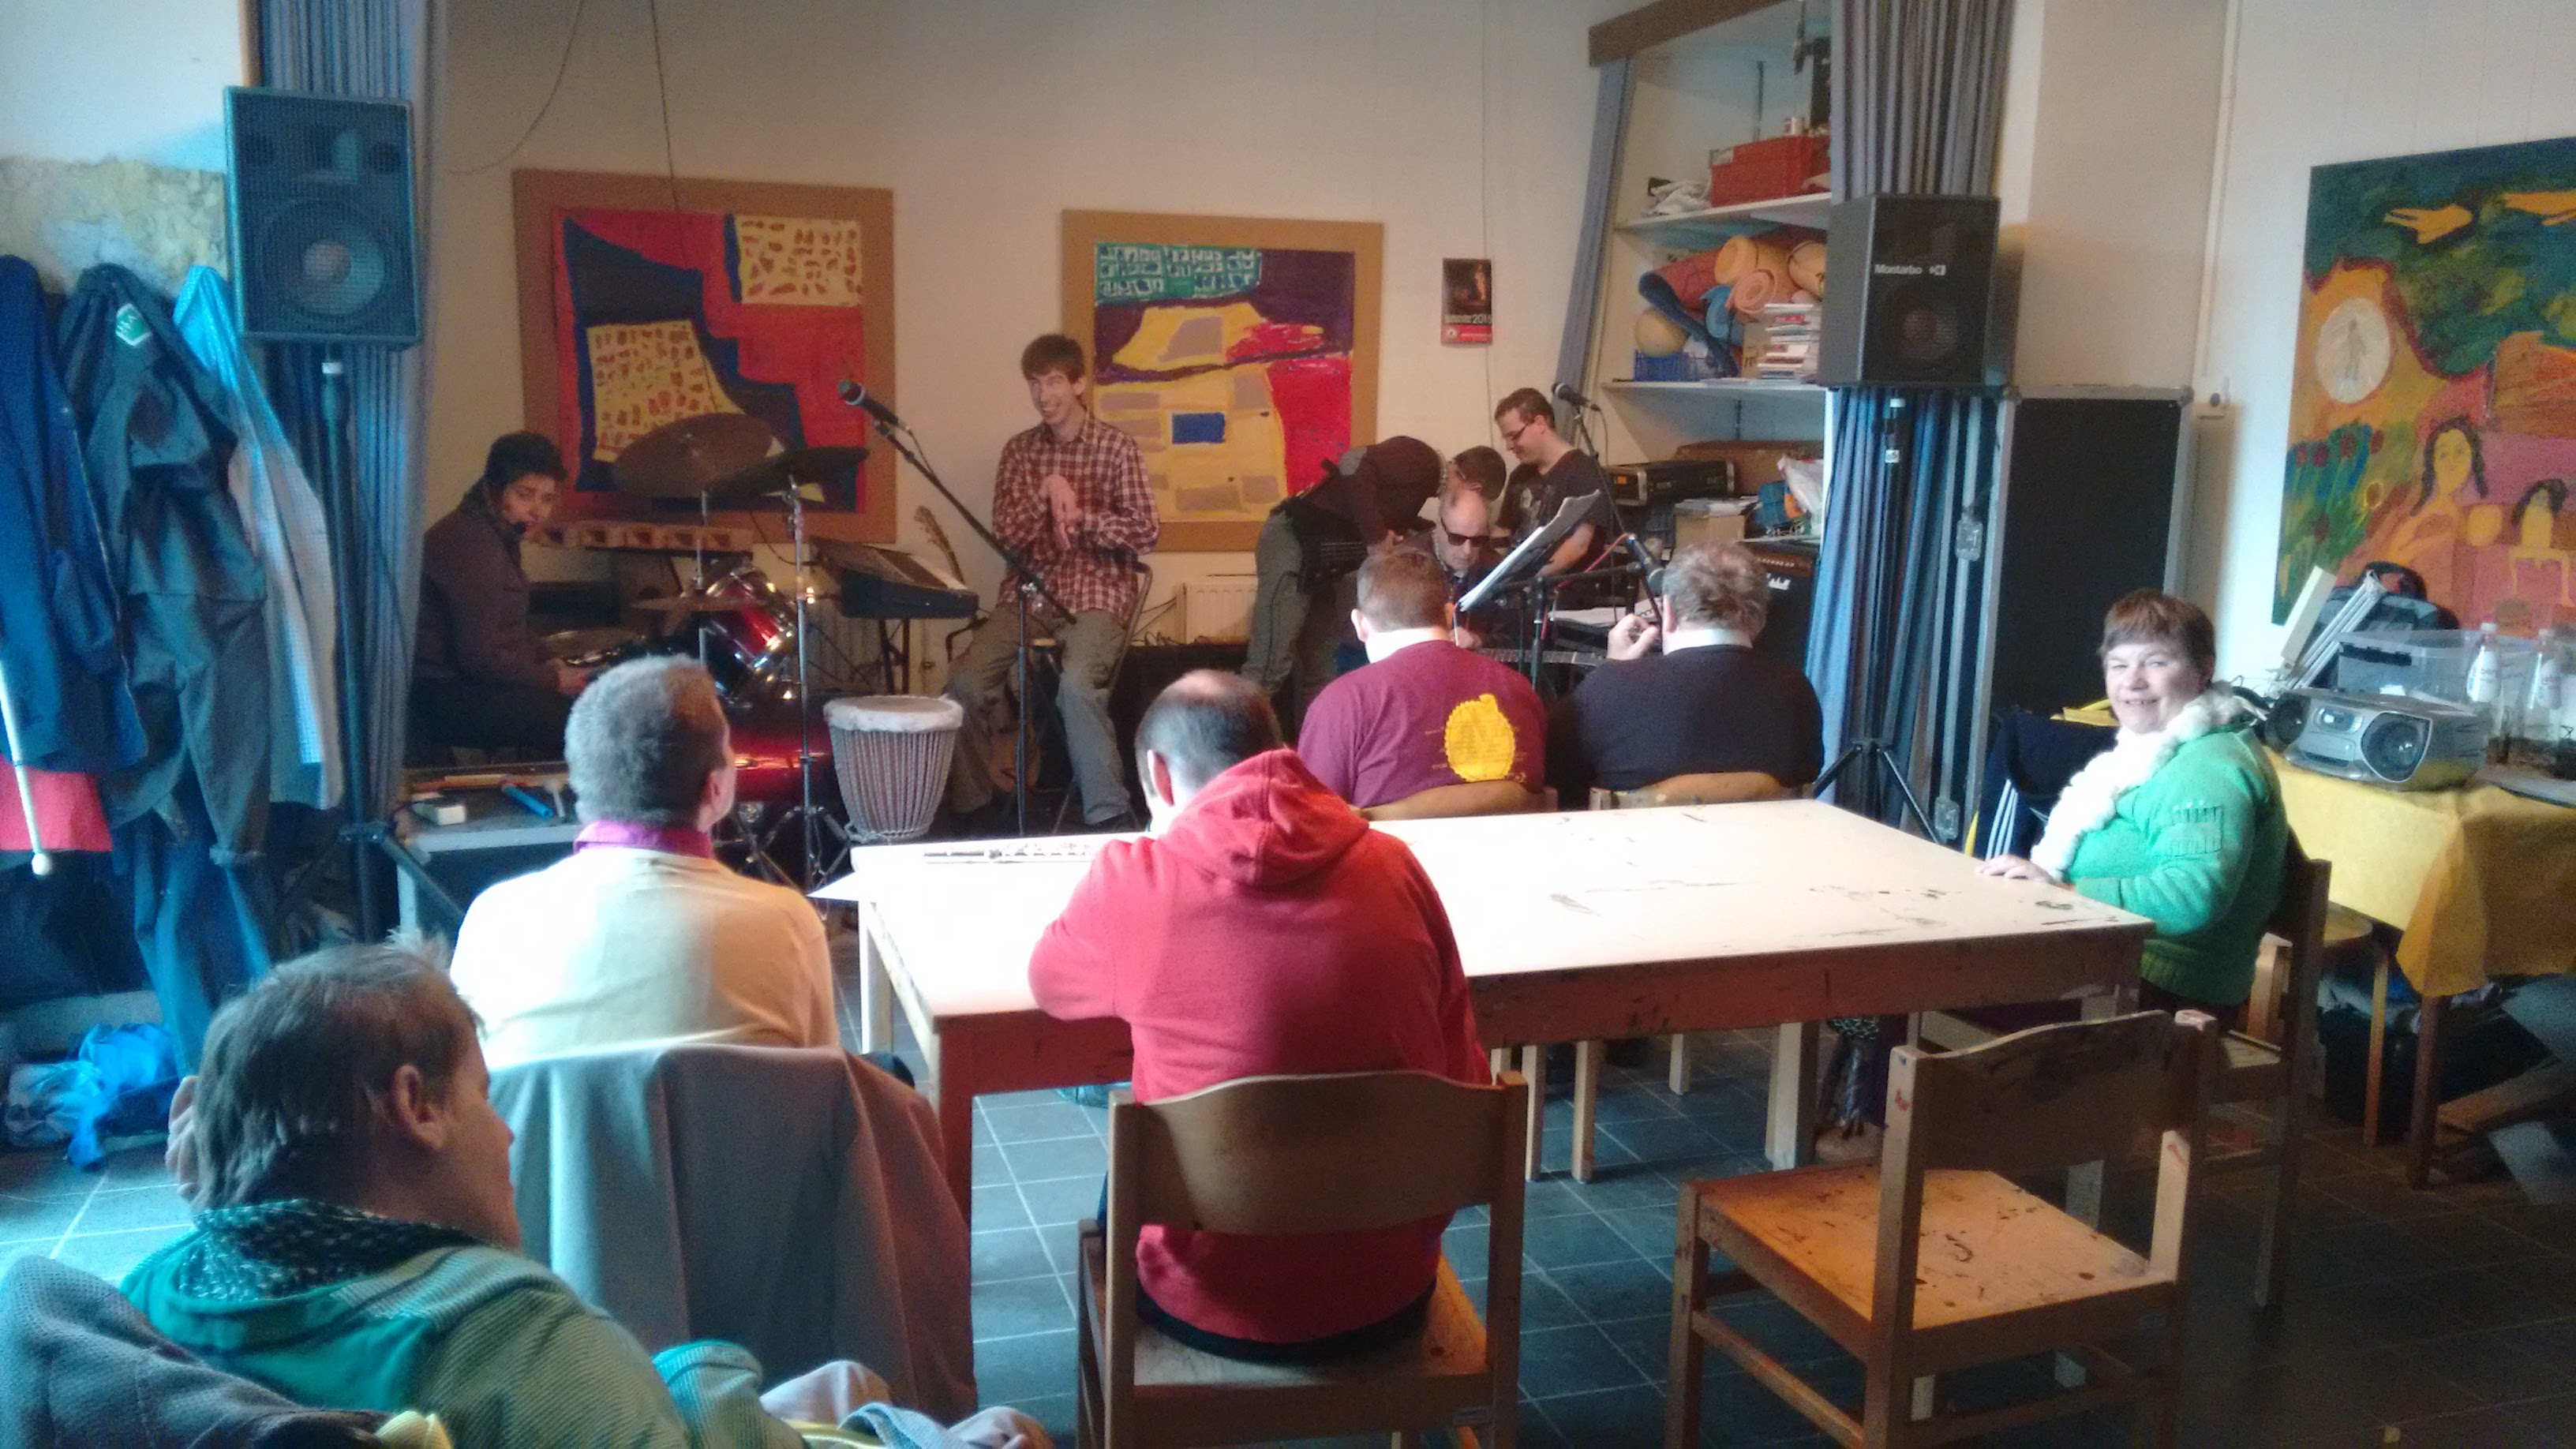
\includegraphics[width=\textwidth]{./muziek.jpg}
  \caption{De groep die muziek maakt tussen twee nummers in}
\end{figure}

Om 11:45 eindigde deze activiteit en heb ik in een andere groep dan gisteren meegeholpen met het eten. Het afwassen gebeurt ook deels met de bewoners, die hier kennelijk wel plezier in hebben, maar niet iedereen vindt dit aangenaam, dus worden ze er niet toe verplicht. Om 13:00 was dit gedaan.

Dan vertelde een bewoners dat hij iets had dat hij mij graag wou laten zien. Hij had namelijk een liedje opgenomen dat op de radio speelde (\emph{Relax - Mika}). Hij genoot er duidelijk van dat hij nu tijd had om wat hij leuk vond te delen met iemand die minder tijdsdruk heeft dan een andere opvoeder.

Daaropvolgend werd hij opgebeld door zijn ouders, waarna hij door ging om de verjaardag van één van de anderen te vieren in de Pizza Hut. Hij vertrok rond 13:20.

\subsubsection{Namiddag}

De namiddag begint zoals elke dinsdagnamiddag met de bewonersvergadering, hierin worden de nieuwigheden van de week, het menu, speciale dingen overlopen door een begeleider, maar ook krijgt elk van de bewoners de kans om hun eigen mening en dingen die volgens hun fout gaan aan te kaarten.

Zo werd er bijvoorbeeld verteld over wie naar hun familie ging over de kerstperiode, iemand die dan op reis zal gaan, een lamp die gebroken was \dots

Ik heb de bewonersvergadering twee keer bijgewoond, want \emph{'t Wit Huis} is opgedeeld in twee \emph{units}, en één van die is nog eens opgedeeld daarbinnen. Dit is omdat er een groot leeftijdsverschil is tussen die twee groepen, en dat dus hun noden anders zijn.

De eerste vergadering duurde tot 15:00, de tweede tot 15:30. Hierna heb ik met enkele van de bewoners gepraat over alledaagse dingen. Daarna stelde een bewoner voor om zijn muziekcollectie te laten horen op zijn kamer.

Die bewoner was een grote fan van Studio Brussel, en ook van \emph{drum and bass}. Toevallig of niet is dit ook mijn lievelingsgenre, dus we praatten hierover voor enkele minuten.

Daarna merkte ik op dat hij een hoop boekjes in braille liggen had. Het leek voor mij alsof ze dezelfde titel hadden, maar blijkbaar gaat het over één boek dat in een hoop hoofdstukken onderverdeeld is. Hij is een van de weinige bewoners die braille kan lezen, omdat de meeste anderen daar het nut niet van inzien. Braille is iets wat je moet blijven onderhouden, anders vergeet je het opnieuw. Het boek is een geschiedenisroman over Keizer Karel en de Gentenaars.

Daarna vertelde hij dat hij ook graag accordeon speelt. Hij is begonnen met accordeon spelen na het overlijden van zijn geleidehond, acht jaar geleden. Hij speelt niet mee in ``De Witte Wolven'', omdat hij niet van die drukte houdt, hij speelt liever alleen. Daarom vindt hij het jammer dat hij zijn accordeon zelf niet kan uithalen, omdat de kans groot is dat hij hem zou laten vallen.

Om 16:40 ga ik weg van bij die bewoner omdat de avondshift begint, en ga ik naar huis.

\subsection{Maandag 21 december 2015}

\section{Ervaringen}

\subsection{Door het personeel}
% halve bladzijde

\subsection{Door mezelf}
% hele bladzijde
Ik heb eigenlijk echt genoten van de stage, het is een ontluchting om te zien hoe bepaalde mensen tevreden kunnen zijn met minder te bereiken. Ze beseffen zelf ook dat ze bijvoorbeeld nooit zullen lezen, maar ze kunnen hun creativiteit kwijt op een hoop verschillende manieren


\end{document}